
\chapter{Background}

\section{Approaches to Software Testing}

% theoretical approaches to software testing with emphasis on GUI testing (robots?)

Software testing is a process of verifying the quality of computer programs to make sure they are
doing what was expected in a consistent, error-free manner. But software testing in practice depends
on \emph{how} and \emph{when} it takes place in the development process. We can distinguish several
types of tests~\cite{tcs,softqualiteng,sta99,emost}. \emph{Unit testing} concentrates on low-level pieces of
software, such as classes and methods. These tests are typically a responsibility of the programmer
transforming the design into implementation. \emph{Acceptance tests} occur at the end of the
development process -- when the software is confronted with its initial requirements specification
and expectations of target users. \emph{Integration tests} (also called \emph{regression tests}),
which we focus on in this paper, happen in between unit and acceptance tests and cover larger blocks
of the program, often the entire product. By running integration tests frequently, we ensure all the
modules work together as a whole and provide results consistent with previously released versions of
the software. Regression tests are thus a quality control aspect -- they allow early detection 
of the program's suspicious behavior caused by changes (refactorings or new features) introduced to 
the product. This kind of constant software testing in anticipation of potential errors is part of most modern 
software development methodologies and is called the \emph{continuous integration}~principle~\cite{fowler}.

Focusing only on GUI testing we may distinguish several techniques specifically designed for this kind of software.
One of more well known and often used approaches is capture-replay which requires some recording tool
for recording all actions performed by a human. The recorded script can be later replayed by the tool, 
thereby repeating the test scenario exactly as it was performed manually. Unfortunately, most of the existing tools
(due to the technical constraints and difficulties) lack the automatic verification module 
leaving this aspect to the tester.

Another technique related to GUI testing (but not only) is called \emph{scripting}. A test case 
recorded using a capture-replay tool usually results in one, long sequence of actions/ events.
The script is really a form of computer program -- a set of instructions for the test tool to act upon.
Having one such program for every test case is not efficient since many test cases share common actions
(such as `show client detail', `go to help screen', etc.). This can lead to higher maintenance costs 
when some aspect of a given action changes. One can cater for this problem by extracting macros and other high-level
programming constructs and build test cases upon these (so that a change only affects one place in the test
scripts).

\section{Review of Existing Testing Frameworks}

We reviewed the existing products (commercial and open source) that somehow tackle
the problem of testing mobile applications in order to see to what extent they allow automated
integration tests. There are very few attempts to solve the problem of mobile software testing.

An open source project \acro{J2MEUnit}~\pcite{j2meunit} can run only simple unit tests. It does not allow
testing application as a whole and the test cases must be written manually. It is also not possible to
integrate \acro{J2MEUnit} into an automatic build process because results of performed tests must be
verified by a human (which excludes its use for integration testing). 
%
Sony Ericsson's \acro{Mobile JUnit}~\pcite{mobilejunit} is a more advanced framework, allowing unit testing on the device and
collecting code coverage statistics automatically while running tests. 
%
\acro{Mobile JUnit} is bound exclusively to the Microsoft Windows operating systems and on-device testing is limited to
Sony Ericsson's telephones. Moreover, the tool's configuration and launching is quite complex and 
involves a pipeline of different tools which cannot be separated. 
%
Recently a few other toolsets similar to Sony's emerged:
\acro{Motorola Gatling}~\pcite{gatling} and \acro{CLDCUnit}~\pcite{cldcunit} for example. The functionality they offer
is close to that of Sony's.

So far we have only mentioned unit testing frameworks. One solution going beyond that point,
towards GUI testing, is IBM's Rational Test RT, in short \acro{TestRT}~\pcite{rational}. \acro{TestRT} is a commercial package
with a custom implementation of unit tests. The program allows GUI testing, but only on so-called
\emph{emulators} (software substitutes of real devices), not on the devices themselves. The simulation
script knows nothing about the emulator or about the mobile environment -- it merely replays
the operating system's events such as keyboard actions or mouse clicks at certain positions over the
emulator window. This implies that the product is testing a software emulation of a real
device rather than the program running on that device. Unfortunately, \acro{Test RT} also lacks an automated test
verification mechanism, the programmer is responsible for checking whether the replayed test passed or not.

A more sophisticated testing solution comes from Research In Motion and is bundled with development
tools for this company's flagship device BlackBerry. The software emulator of a BlackBerry device
(called \acro{Fledge}~\pcite{bbfledge}) is equipped with a controller tool that can interpret
predefined event scripts. These scripts can contain events such as: starting and pausing the
application, changing the readouts of \acro{GPS} location \acro{API} for devices supporting \acro{GPS} positioning,
generating keypad and other input device events, generating various phone events such as remote
phone calls or changing battery level. BlackBerry's controller has several limitations: it runs only
with the simulator, not with real devices, it lacks an automated test verification mechanism
(assertions) and, most of all, the developers are unable to record test scenarios -- all scripts
must be written by hand prior to testing.

The conclusion from the list above is that in spite of the evolving theory of GUI testing,
practical implementations for testing mobile applications remain within the domain of the simplest
unit and limited GUI tests.

\section{J2ME Architecture}

% a short presentation of J2ME architecture, emphasizing GUI specifics
{\itshape\small This chapter was written based on material in the following
literature and on-line resources: \cite{midpspec,j2mecrackingcode,enterprisej2me,j2mereference,midpstyle}.}

\bigskip%
Sun Microsystems defines J2ME as \emph{a highly optimized Java runtime environment targeting
a wide range of consumer products, including pagers, cellular phones, screen-phones,
digital set-top boxes and car navigation systems}.
Announced in June 1999 at the JavaOne Developer Conference, J2ME brings the
cross-platform functionality of the Java language to smaller devices, allowing mobile
wireless devices to share applications. With J2ME, Sun has adapted the Java platform for
consumer products that incorporate or are based on small computing devices.

The J2ME architecture comprises three layers. The first layer
is the configuration layer that includes the Java Virtual Machine (JVM), which directly
interacts with the native operating system. The configuration layer also handles interactions
between the profile and the JVM. The second layer is the profile layer, which
consists of the minimum set of application programming interfaces (APIs) for the small
computing device. The third layer is the Mobile Information Device Profile (MIDP).
The MIDP layer contains Java APIs for user network connections, persistence storage,
and the user interface. It also has access to CLDC libraries and MIDP libraries.

J2ME uses configurations and profiles to customize the Java Runtime Environment (JRE) 
and tailor it to the capabilities of hardware devices.
As a complete Java runtime environment, J2ME consists of a configuration which determines the JVM used 
and a profile which defines the application by adding domain-specific classes to the J2ME
configuration to define certain uses for devices. The configuration defines the basic
run-time environment as a set of core classes and a specific JVM that run on specific types
of devices.

Figure~\ref{fig:j2mearchitecture} depicts the relationship between different virtual machines,
configurations, and profiles. It also draws a parallel with the J2SE API and its Java virtual
machine. While the J2SE virtual machine is generally referred to as a JVM, the J2ME virtual
machines, KVM and CVM, are subsets of JVM. Both KVM and CVM can be thought of as a
kind of Java virtual machine -- they are shrunken versions of the J2SE JVM and
are specific to J2ME.

\begin{figure}[t]%
\begin{center}
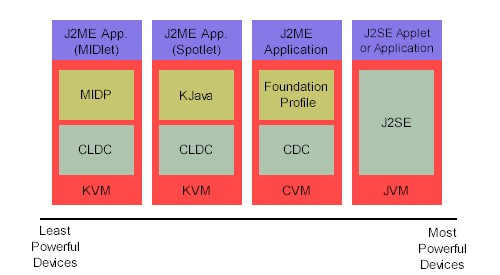
\includegraphics[width=.8\linewidth]{figures/j2me-architecture}
\end{center}
\caption{J2ME Architecture (from: `J2ME: Step by step' by IBM developerWorks).}%
\label{fig:j2mearchitecture}
\end{figure}

The modular design of the J2ME architecture enables an application to be scaled based on
constraints of a small computing device. J2ME architecture does not replace the operating
system of a small computing device. Instead, J2ME architecture consists of layers located
above the native operating system, collectively referred to as the Connected Limited
Device Configuration (CLDC). The CLDC, installed on top of the operating
system, forms the run-time environment for small computing devices.

\begin{figure}[t]%
\begin{center}
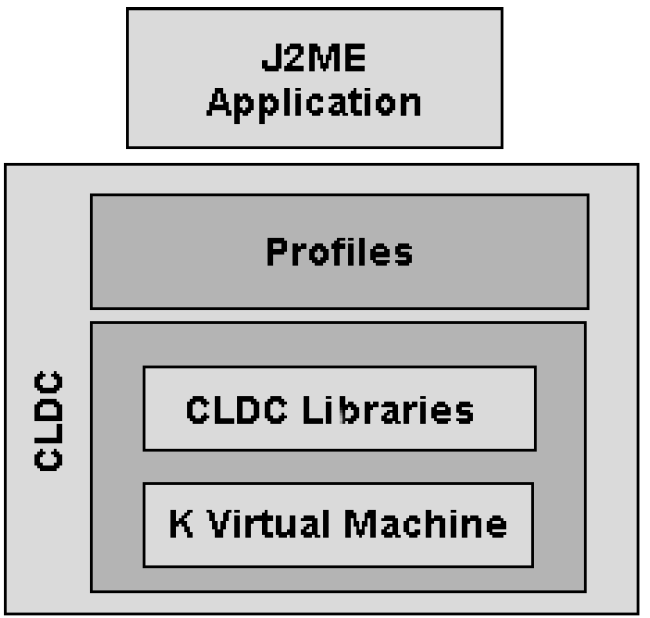
\includegraphics[height=6cm]{figures/j2me-architecture-2-b}
\end{center}
\caption{J2ME Architecture cd (from: `Wireless Programming with J2ME: Cracking the Code' by Dreamtech Software India, Inc., Team).}%
\label{fig:j2mearchitecture2}
\end{figure}

A \emph{MIDlet} is a J2ME application designed to operate on an MIDP small computing
device. A MIDlet is defined with at least a single class that is derived from the 
\texttt{javax\-.microedition\-.midlet\-.MIDlet} class.

\subsection{Event Handling}

A MIDlet is an event-based application. All routines executed in the MIDlet are invoked
in response to an event reported to the MIDlet by the application manager. The initial
event that occurs is when the MIDlet is started and the application manager invokes the
\texttt{startApp()} method.

The \texttt{startApp()} method in a typical MIDlet contains a statement that displays a screen
of data and prompts the user to enter a selection from among one or more options. The
nature and number of options is MIDlet and screen dependent.

A \texttt{Command} object is used to present a user with a selection of options to choose
from when a screen is displayed. Each screen must have a \texttt{CommandListener}. A \texttt{CommandListener}
monitors user events with a screen and causes the appropriate code to execute based on the current event.

\subsection{User Interfaces}

The design of a user interface for a MIDlet depends on the restrictions of a small
computing device. Some small computing devices contain resources that provide
a rich user interface, while other more resource-constrained devices offer a modest
user interface. A rich user interface contains the following elements, and a device
with a minimal user interface has some subset of these elements as determined by
the profile used for the device.

A \texttt{Form} is the most commonly invoked user interface element found in a MIDlet
and is used to contain other user interface elements. Text is placed on a form as a
\texttt{StringItem}, a \texttt{List}, a \texttt{ChoiceGroup}, and a \texttt{Ticker}.

A \texttt{StringItem} contains text that appears on a form that cannot be changed by the
user. A \texttt{List} is an itemized options list from which the user can choose an option. A
\texttt{ChoiceGroup} is a related itemized options list. And a \texttt{Ticker} is text that is scrollable.

A user enters information into a form by using the \texttt{Choice} element, \texttt{TextBox},
\texttt{TextField}, or \texttt{DateField} elements. The \texttt{Choice} element returns an option that the user
selected. \texttt{TextBox} and \texttt{TextField} elements collect textual information from a user and
enable the user to edit information that appears in these user interface elements. The
\texttt{DateField} is similar to a \texttt{TextBox} and \texttt{TextField} except its contents are a date and time.

An \texttt{Alert} is a special case of a \texttt{Form} that is used to alert the user that an error has occurred.
An \texttt{Alert} is usually limited to a \texttt{StringItem} user interface element that defines the
nature of the error to the user.

To use the display and the low-level user interface API directly, the developer should use the \texttt{Graphics}
and \texttt{Canvas} classes.
The \texttt{Canvas} class provides the display surface, its dimensions, and callbacks used to handle key and pointer events
and to paint the display when requested. The methods of this class must be overridden by the developer to respond
to events and to paint the screen when requested. The \texttt{Graphics} class provides methods to paint lines, rectangles,
arcs, text, and images to a \texttt{Canvas} or an \texttt{Image}. To gain access to even more low-level events a programmer
can use \texttt{GameCanvas} class that is direct subclass of Canvas.
